% !TEX root = MAIN.tex
\chapter{Graphtheory}\label{sec:geo}
graphs are networks of dots and lines. They have nothing in commom with graphs of function.

it presents under a different aspect.
intuitively accessible

kids should be aware of applications

\section{Historical Remarks}\label{sec:geoobj}
The Bridge Problem
find a tour crossing every bridge exactly once 
Leonhard Euler 1735
K\"onigsberger Br\"ucken Problem
K\"onigsberg. The medieval city is now Kaliningrad. The city 

The Pregel river goes through this town, which has two large islands in the middle. These islands are surrounded by the river. The islands are connected by seven bridges as shown in picutre .
Karl Leonhard Gottlieb Ehler came up with the question, which route has one to take to cross all seven bridges without crossing any of them more than once? Carl struggled with this problem and decided to write the famous mathematician Leonard Euler for help.
Leonard Euler invented a new field in mathematics. The Geometry of Position, now known as gtapg theory.
The four landmasses can be simplified by four nodes, and lines between them to represent the bridges.
degree of each node is the number 
beginn and the end of the path
Picture 
Eulerian Cycle Problem: Find a cycle that visists every edge exactly once (linear)
Hamiltonian Cycyle Problem: find a cycle that visits every vertex exactly once (NP)

This is known as Euler's Theorem:
    A connected graph has an Euler cycle if and only if every vertex has even degree.

In this given real-world situation we can represent our problem with a graph model.
Let each country be a vertex where vertices are adjacent if they share a border.    
    
\begin{definition}
  This is a definition.
  A graph G is a set V of vertices, and a set E of edges. The set E contains pairs of distinct elements of V.
\end{definition}    
    
\section{Mathematical Graphtheory}\label{sec:works}
The difinitions and informations in the following sections are taken from the book ...
Mathematische Beschreibung der Graphentheorie
In graph theory, a cycle in a graph is a non-empty trail in which only the first and last vertices are equal.
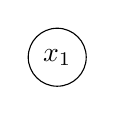
\begin{tikzpicture}[main/.style = {draw, circle}] 
\node[main] (1) {$x_1$}; 
\end{tikzpicture} 

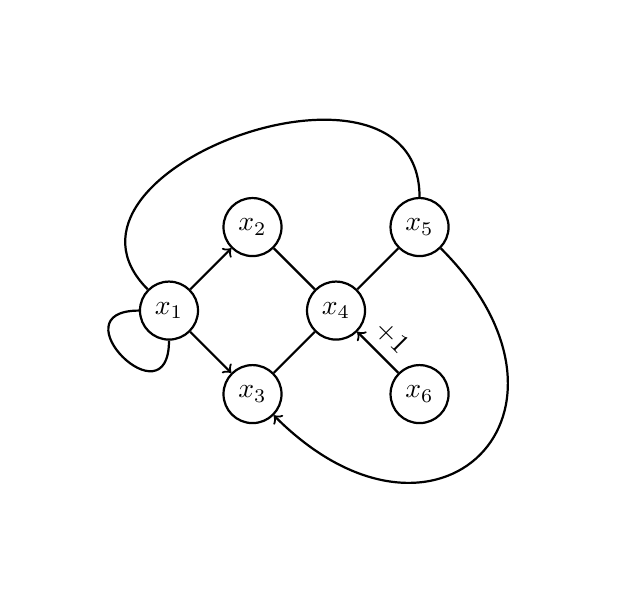
\begin{tikzpicture}[node distance={15mm}, thick, main/.style = {draw, circle}] 
\node[main] (1) {$x_1$}; 
\node[main] (2) [above right of=1] {$x_2$}; 
\node[main] (3) [below right of=1] {$x_3$}; 
\node[main] (4) [above right of=3] {$x_4$}; 
\node[main] (5) [above right of=4] {$x_5$}; 
\node[main] (6) [below right of=4] {$x_6$}; 
\draw[->] (1) -- (2); 
\draw[->] (1) -- (3); 
\draw (1) to [out=135,in=90,looseness=1.5] (5); 
\draw (1) to [out=180,in=270,looseness=5] (1); 
\draw (2) -- (4); 
\draw (3) -- (4); 
\draw (5) -- (4); 
\draw[->] (5) to [out=315, in=315, looseness=2.5] (3); 
\draw[->] (6) -- node[midway, above right, sloped, pos=1] {+1} (4); 
\end{tikzpicture} 

\begin {center}
\begin {tikzpicture}[-latex ,auto ,node distance =4 cm and 5cm ,on grid ,
semithick ,
state/.style ={ circle ,top color =white , bottom color = processblue!20 ,
draw,processblue , text=blue , minimum width =1 cm}]
\node[state] (C)
{$1$};
\node[state] (A) [above left=of C] {$0$};
\node[state] (B) [above right =of C] {$2$};
\path (A) edge [loop left] node[left] {$1/4$} (A);
\path (C) edge [bend left =25] node[below =0.15 cm] {$1/2$} (A);
\path (A) edge [bend right = -15] node[below =0.15 cm] {$1/2$} (C);
\path (A) edge [bend left =25] node[above] {$1/4$} (B);
\path (B) edge [bend left =15] node[below =0.15 cm] {$1/2$} (A);
\path (C) edge [bend left =15] node[below =0.15 cm] {$1/2$} (B);
\path (B) edge [bend right = -25] node[below =0.15 cm] {$1/2$} (C);
\end{tikzpicture}
\end{center}
